
\section{Data visualization}

\subsection{MRI Image}
\begin{figure}
    \centering
    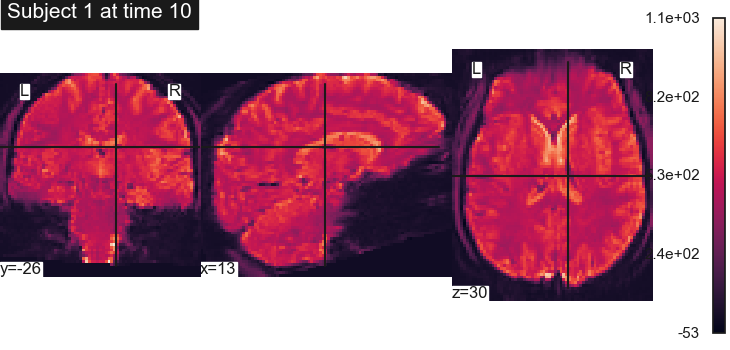
\includegraphics[width=\textwidth]{img/example_fmri.png}
    \caption{Example of a 3D MRI plotted for the first patient}
    \label{fig:ex_mri}
\end{figure}

\subsection{Time series diagnosis}
\begin{figure}
    \begin{subfigure}{\textwidth}
        \centering
        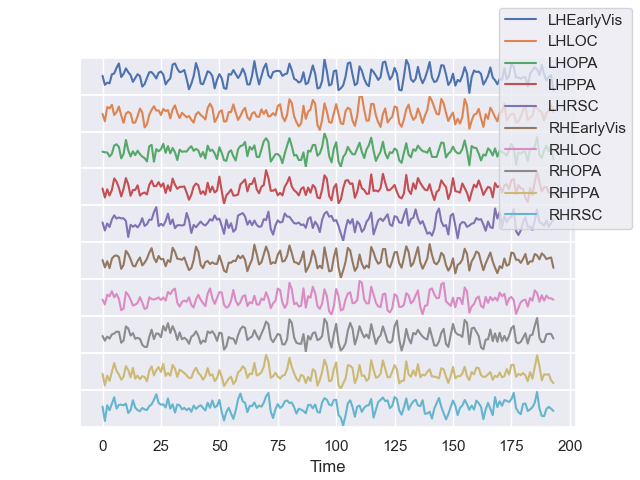
\includegraphics[height=.4\textheight]{img/plot_time_series.png}
        \caption{Time series in each region of interests}
        \label{fig:plot_TS}
    \end{subfigure}
    \begin{subfigure}{\textwidth}
        \centering
        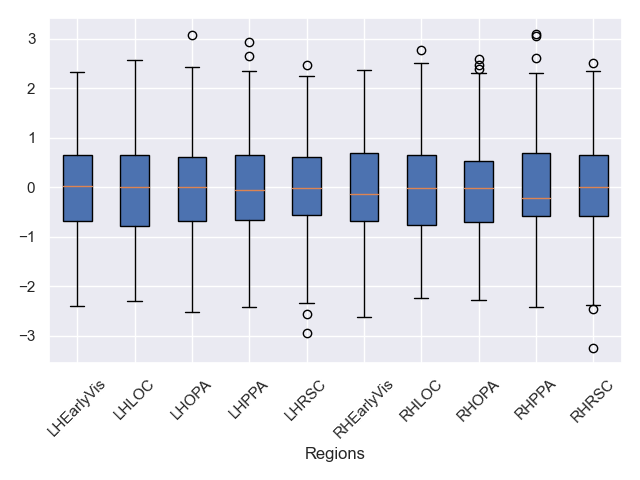
\includegraphics[height=.4\textheight]{img/boxplot_time_series.png}
        \caption{Box plot of the time series}
        \label{fig:boxplot_TS}
    \end{subfigure}
    \caption{Analysis of the extracted time series. There were 10 ROIs: early visual (EarlyVis), lateral occipital cortex (LOC), occipital place area (OPA), parahippocampal place area (PPA), retrosplenial complex (RSC) for the left hemisphere (LH) and right hemisphere (RH).} 
    \label{fig:analysis_TS}
\end{figure}

\begin{figure}
    \centering
    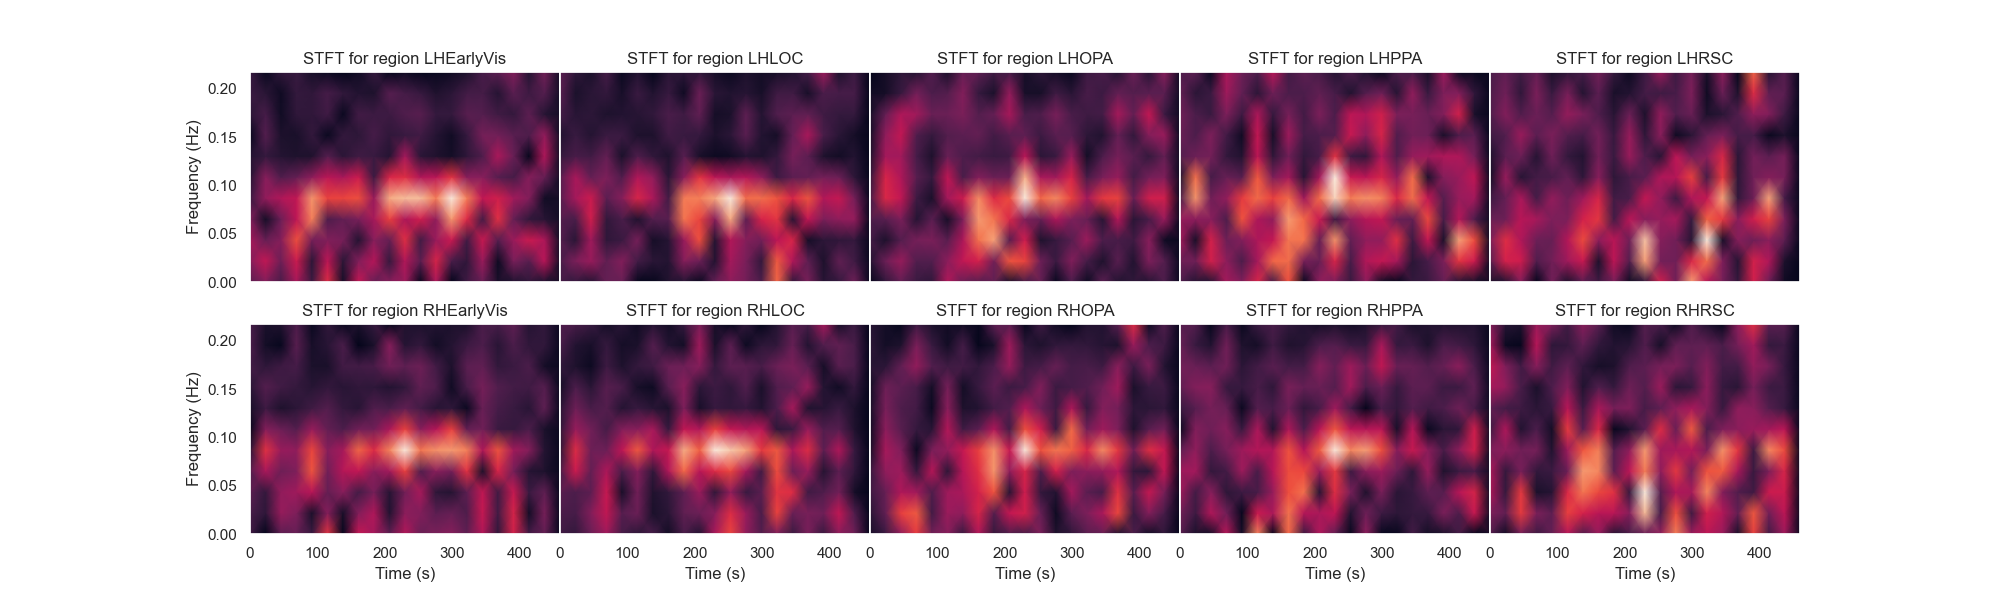
\includegraphics[width=\textwidth, height=0.25\textheight]{img/autocorrelation_TS.png}
    \caption{Autocorrelation analysis across various brain regions. Not all results were plotted to enhance readability.}
    \label{fig:autocorr_TS}
\end{figure}

\begin{figure}
    \centering
    \begin{subfigure}{\textwidth}
        \centering
        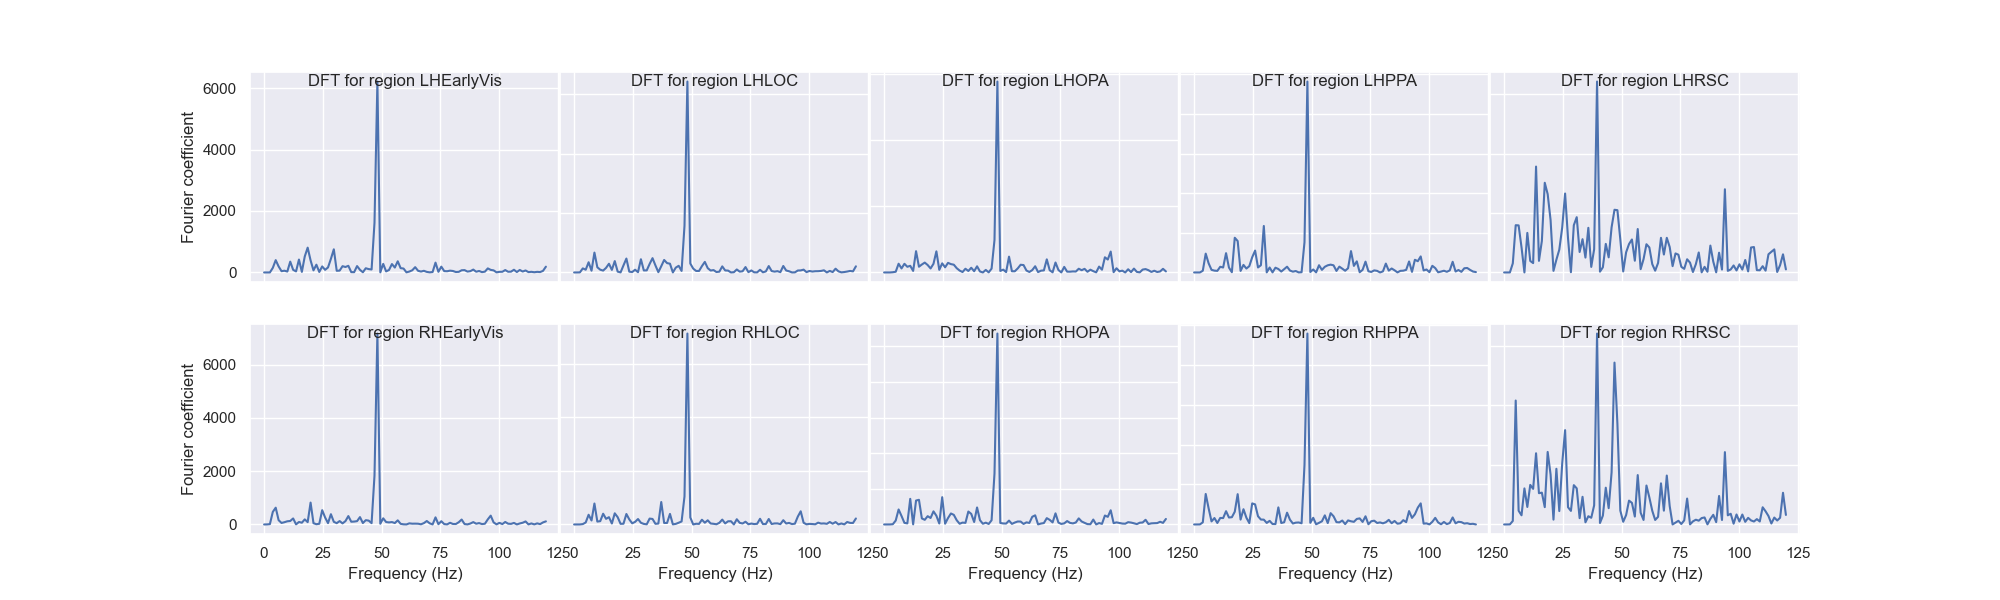
\includegraphics[width=\textwidth, height=0.28\textheight]{img/DFT_TS.png}
        \caption{Discrete Fourier Transform (DFT)}
    \end{subfigure}
    \begin{subfigure}{\textwidth}
        \centering
        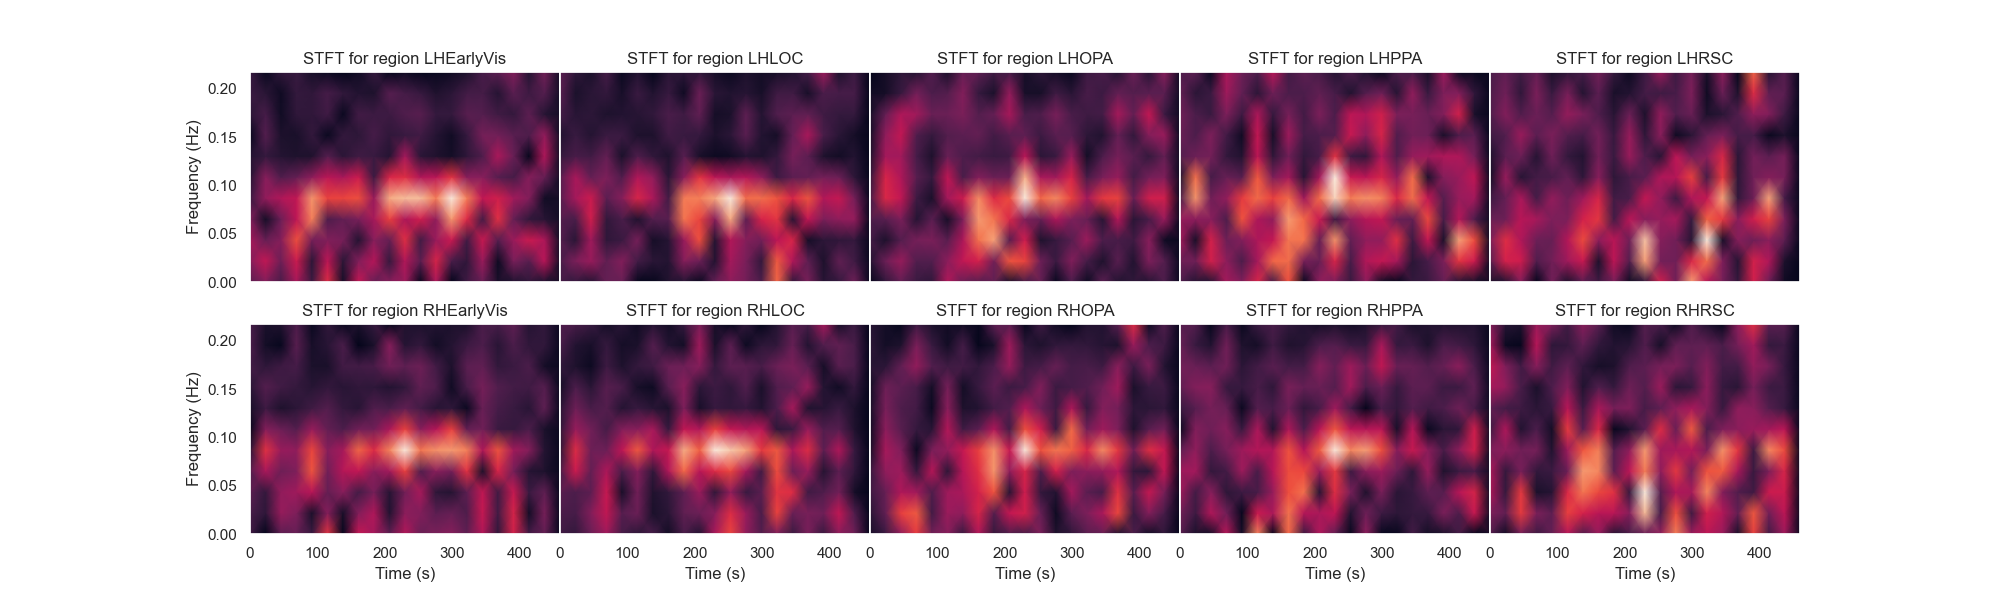
\includegraphics[width=\textwidth, height=0.25\textheight]{img/spectrogram_TS.png}
        \caption{Spectrogram}
        \label{spectrogram_TS}
    \end{subfigure}
    \caption{Spectral analysis of the time series for each brain region. (b) The spectrogram was computed with window length of $20$ and an overlapping of $16$.}
    \label{fig:spectral_TS}
\end{figure}

\section{Graph Construction}

\begin{figure}[H]
\centering
    \begin{subfigure}{\textwidth}
        \centering
        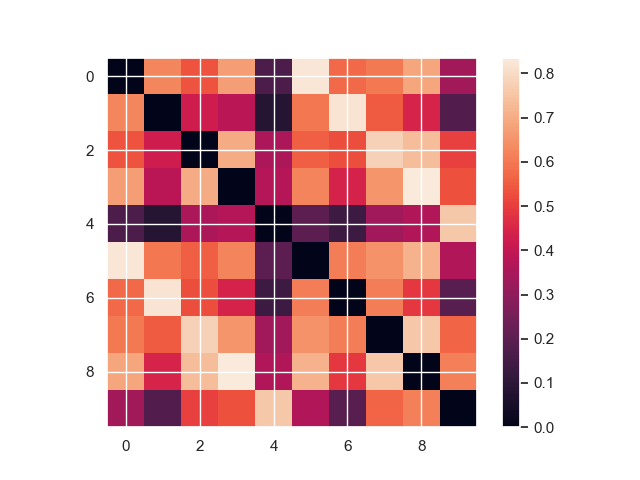
\includegraphics[height=.35\textheight]{img/connectivity_matrix.png}
        \caption{Connectivity matrix}
        \label{fig:connectivity}
    \end{subfigure}
    \begin{subfigure}{\textwidth}
        \centering
        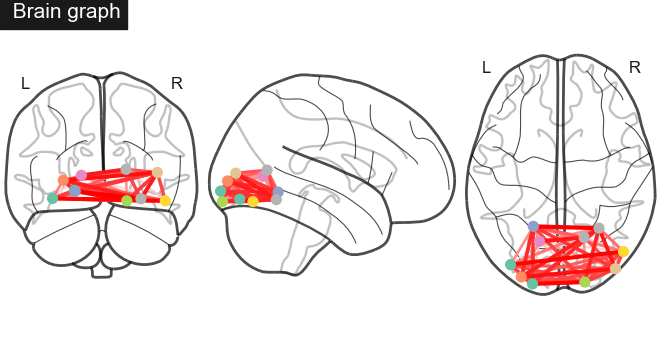
\includegraphics{img/brain_graph.png}
        \caption{Functional-connectome graph}
        \label{ex_graph}
    \end{subfigure}
    \caption{Representation of the brain graph. (a) Connectivity matrix for a given patient, which is also the adjacency matrix $\A$ of the graph $\G$. The entry $A_{i,j}$ of the connectivity matrix is obtained by computing the correlation coefficient between the time series extracted from regions $i$ and $j$. (b) displays the corresponding \textit{connectome}. This representation offers a unique insight into the patient’s
neural architecture, highlighting the potential correlates of cognitive processes}
    \label{fig:brain_graph}
\end{figure}

% \begin{figure}
%     \centering
%     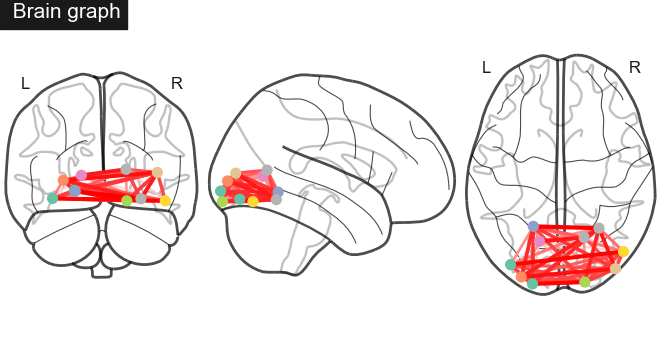
\includegraphics{img/brain_graph.png}
%     \caption{Caption}
%     \label{fig:enter-label}
% \end{figure}
